I dette afsnit vil vi definere Riemann-integralet.\footnote{Afsnittet er primært baseret på \cite{Abbott2002}, s. 183-194}
Det skal dog bemærkes, at vi ikke benytter Riemanns originale definition, men derimod en videreudvikling af den franske matematiker Darboux.
Det kan bevises, at de to definitioner på integralet er ækvivalente.\footnote{\cite{Bartle2010}, s. 231-232.}

Vi starter med nogle grundlæggende definitioner, vi har brug for til at definere integralet.
\begin{definition}{Inddeling}{}
  Antag $a,\;b \in \mathbb{R}$ sådan at $a <b$.
  Ved en inddeling $P$ af $[a;b]$ forstår vi en endelig mængde $\{x_0,\dotsc, x_n\}$, hvor
  \[
  a=x_0<x_1<\cdots<x_n=b
  \] 
  og vi skriver 
  \[
  \Delta x_i=x_i-x_{i-1} \quad (i=1,\ldots ,n)
  \]  
\end{definition}
Med en inddeling kan vi dele intervallet $[a;b]$ op i $n$ delintervaller, hvor det $i$'te delinterval har længden $\Delta x_i$:
\[
[a;b]=[x_0;x_1] \cup [x_1;x_2]\cup \cdots \cup [x _{n-1};x_n]
\] 
Vi vil nu definere over- og undersummen af en funktion med hensyn til en given inddeling.

\begin{definition}{Over- og undersum}{}
  Antag $f:[a;b] \to \mathbb{R}$ er en begrænset funktion, og $P=\{x_0,\ldots, x_n\}$ er en inddeling af $[a;b]$. 
  Lad 
  \[
  M_i=\sup \{ f(x):x \in [x _{x_{i-1}};x_i] \} \quad{\text{og}} \quad m_i=\inf \{ f(x):x \in [x _{x_{i-1}};x_i] \}.
  \] 
  Så er oversummen af $f$ med hensyn til $P$ defineret ved
  \[
  U(f,P)=\sum_{i=1}^{n} M_i \Delta x_i.
  \] 
  Tilsvarende er undersummen af $f$ med hensyn til $P$ defineret ved
  \[
  L(f,P)=\sum_{i=1}^{n} m_i \Delta x_i.
  \] 
\end{definition}

Vi kræver i definitionen, at $f(x)$ er begrænset, da vi så fra sætning \ref{theo:supremum-egenskab} ved, at $M_i$ og $m_i$ eksisterer. 

\begin{theorem}[label=theo:ulighed_overundersum]{Uligheder med over- og undersummer}{}
  Antag $f:[a;b] \to \mathbb{R}$ er en begrænset funktion og $P$, $P'$ er inddelinger af $[a;b]$ sådan at $P \subseteq P'$. Så gælder
  \[
  L(f,P)\leq L(f,P') \text{ og }  U(f,P') \leq U(f,P).
  \] 
\end{theorem}
\begin{proof} 
  \footnote{Beviset er baseret på \cite{Axler2020}, s. 3-4.} 
  Lad $P=\{ x_0,\ldots , x_n \} $ og $P'=\{x_0',\ldots x_N'\}$. 
  Siden $P \subseteq P'$, så har vi, at for hver $j=1,\ldots , n$ eksisterer $k \in \{ 0,\ldots , N-1 \} $ og $m \in \mathbb{Z}^+$ sådan at $x _{j-1} =x_k'< \cdots < x _{k+m}'=k_j$.

  Så gælder for hver $i=1, \ldots , m$, at ${\{ f(x):x \in [x'_{k+i-1};x'_{k+i }] \} \subseteq \{ f(x):x \in [x_{j-1},x_j]\}  }$, og 
  \begin{equation*}
  \begin{split}
   m_j&=\inf \{ f(x):x \in [x_{j-1};x_j]\} \\
    &\leq  \inf \{ f(x):x \in [x'_{k+i-1};x'_{k+i }] \}\\
    &=m'_{k+i}.
  \end{split}
  \end{equation*}
Vi får så uligheden 
\begin{equation*}
\begin{split}
  m_j \Delta x_j&=\sum_{i=1}^{m} m_j \Delta x _{k+i}\\
  &\leq \sum_{i=1}^{m} m' _{k+i} \Delta x _{k+i}.
\end{split}
\end{equation*}
  Det følger, at $L(f,P) \leq L(f,P')$. 

  Tilsvarende har vi for hver $i=1,\ldots, m$ også, at
  \begin{equation*}
  \begin{split}
    M_j&=\sup \{ f(x):x \in [x_{j-1};x_j] \} \\
    &\geq \sup \{ f(x):x \in [x'_{k+i-1};x'_{k+i}] \} \\
    &=M'_{k+i},
  \end{split}
  \end{equation*}
  og vi får uligheden
  \begin{equation*}
  \begin{split}
  M_j \Delta x_j&=\sum_{i=1}^{m} M_j \Delta x _{k+i}\\
  &\leq \sum_{i=1}^{m} M' _{k+i} \Delta x _{k+i}.
  \end{split}
  \end{equation*}
  Det følger, at $U(f,P) \geq U(f,P')$
\end{proof}

Beviset for sætning \ref{theo:ulighed_overundersum} kan godt virke uoverskueligt grundet notationen, men \cref{fig:ulighed_overundersum} tydeliggør i høj grad ideen i beviset.

\begin{figure}[H]
\begin{center}
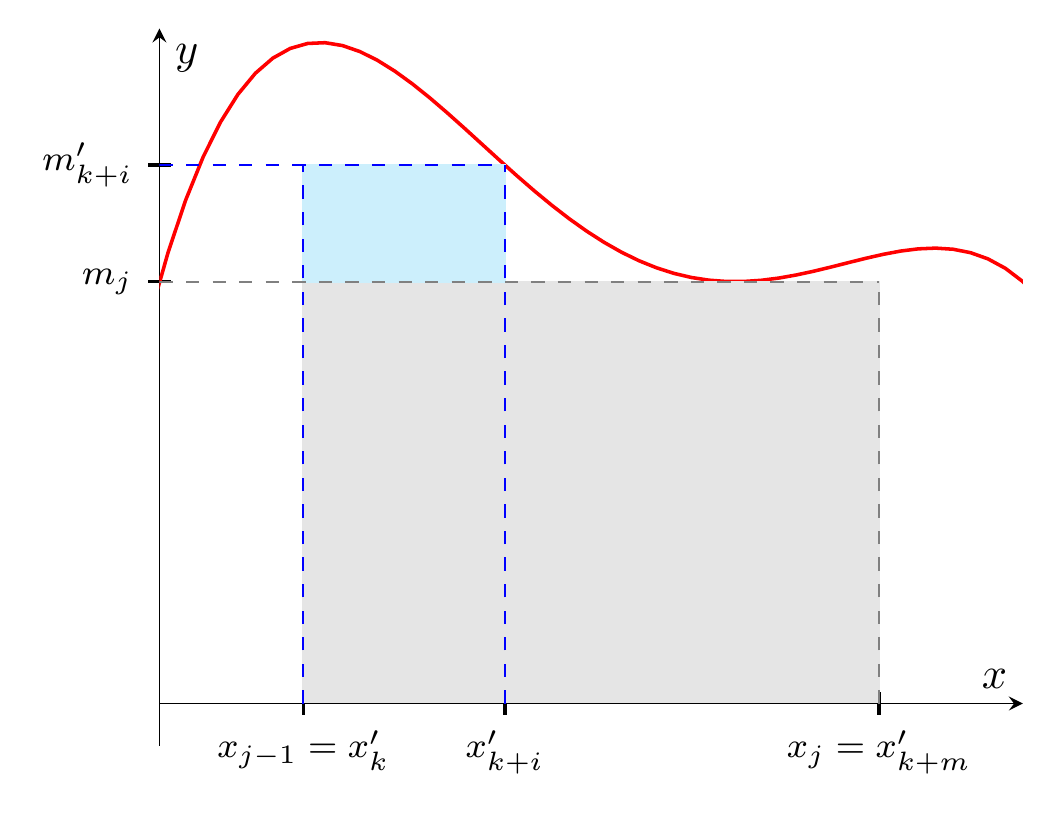
\begin{tikzpicture}[scale=1.6, transform shape]
\begin{axis}[xmin=0, xmax=3, ymin=-0.5, ymax=8, axis lines=middle,
  xlabel=$x$,ylabel=$y$,
  xtick={0.5,1.2,2.5},
  xticklabels={$x _{j-1}=x'_{k}$, $x'_{k+i}$, $x_j=x'_{k+m}$},
  xticklabel style={anchor=north, font=\footnotesize},
  ytick={6.3824,5},
  yticklabels={$m'_{k+i}$, $m_j$},
  every major tick/.append style={thick, major tick length=5pt, black},
  yticklabel style={anchor=east, font=\footnotesize}
  ]
  \addplot[color=red, domain=-1:5, samples=100, thick]{-(x-2)^4 - (x-2)^3 + 2*(x-2)^2+5} node[left, pos=0.15] {$f$};
  \filldraw[gray!20] (axis cs:0.5,0.02) rectangle (axis cs:2.5,5);
  \filldraw[cyan!20] (axis cs:0.5,5) rectangle (axis cs:1.2,6.3824);
  \draw[color=blue, dashed] (axis cs:0.5,0) -- (axis cs:0.5,6.3824);
  \draw[color=blue, dashed] (axis cs:0,6.3824) -- (axis cs:1.2,6.3824);
  \draw[color=gray, dashed] (axis cs:2.5,0) -- (axis cs:2.5,5);
  \draw[color=gray, dashed] (axis cs:0,5) -- (axis cs:2.5,5);
  \draw[color=blue, dashed] (axis cs:1.2,0) -- (axis cs:1.2,6.3824);
\end{axis}
\end{tikzpicture}
\end{center}
  \caption{Ideen i beviset af sætning \ref{theo:ulighed_overundersum}}%
\label{fig:ulighed_overundersum}
\end{figure}

